\documentclass{article}

\usepackage{graphics}
\usepackage{graphicx}
\usepackage[a4paper,
            top=2cm,
            bottom=3cm,
            left=3cm,
            right=2cm,
            marginparwidth=1.75cm
            ]{geometry}

\usepackage{float}
\usepackage{subcaption}

\title{TP02 - Estrutura de dados}
\author{Marcos Daniel Souza Netto - 2022069492} 
\date{\today}

\begin{document}
\maketitle

\section{Introdução}

O problema proposto consiste em implementar um programa que recebe um grafo 
e a coloração dos seus vértices e verifica se a coloração dada é gulosa, ou seja,
todo vertíce deve possuir a cor $i$ somente se existir vertices adjacentes
a ele com cores $1, 2, ..., i-1$. Por fim, também deve ser retornada a permutação
dos vértices utilizada na coloração gulosa, isto é, apresentar como o grafo foi 
colorido, apresentando os vértices de cor $k$ seguidos dos vértices de cor $k + 1$, 
os vértices de cada cor devem estar ordenados pelo seu rótulo.

A solução implementada leva em consideração a quantidade de vértices mínima de diferentes cores, 
menor que a cor do vértice analisado, para que a coloração seja gulosa. Observe que para satisfazer 
condição de gulosidade é necessário que cada vértice de cor $i$ tenha pelo menos $i-1$ vértices adjacentes 
de cores menores que $i$. Para isso, foi utilizada a estrutura de dados \textbf{set}, tal que para \underline{todo} vértice
de cor menor que $i$, é inserido sua cor no set, e depois de passar por todos essas cores, é verificado se o tamanho do set 
é menor que $i-1$, caso seja, a coloração não é gulosa.

Para a parte da permutação usada, apenas foi utilizada a ordenação escolhida de modo que a comparação entre dois vértices é feita 
pelo sua cor primeiramente, e caso sejam iguais, é feita a comparação pelo seu rótulo. Observe que aqui, ao utilizar do par ordenado, cor e rótulo, 
o par ordenado se torna única uma vez que a utilização do rótulo já garante unicidade. Desse maneira, métodos de ordenação não estáveis (que pode não preservar a ordem dos elementos iguais) retornam 
a mesma solução. 

\section{Método}

A seguir serão detalhados a implementação da solução, de modo a explicitar 
as estruturas de dados utilizadas e as estratégias de solução. A priori vale 
apresentar as especificações do ambiente de desenvolvimento utilizado:

\begin{itemize}
    \item Sistema Operacional: Ubuntu 22.04.3 LTS;
    \item Compilador: G++ 11.4.0;
    \item Processador: Ryzen 5 5500u;
    \item Memória RAM: 8GB.
\end{itemize}


\subsection{Estruturas de dados}

Em síntese, foram utilizadas as seguintes estruturas de dados:

\begin{itemize}
    \item \textbf{set}: Estrutura de dados que armazena elementos únicos, e que permite a inserção, remoção e busca em tempo $O(log(n))$ (Se tratássemos de uma árvore balanceada, mas aqui não tem esse tipo de tratamento, logo essa estrutura tem complexidade $O(n)$ no pior caso), 
    para tanto ela foi implementada como uma árvore binária de busca, e foi utilizada para armazenar as cores dos vértices adjacentes;    

    \item \textbf{vector}: Estrutura de dados que armazena elementos em sequência contínua de memória. Foi utilizada para representar o grafo, 
    ou seja, o grafo aqui foi representado como um vetor de listas de adjacências, onde cada posição do vetor representa um vértice, tal que cada 
    posição possui um subvetor contendo os vértices adjacentes a ele;

    \item \textbf{pair}: Tipo abstrato de dados que generaliza a ideia de um par ordenado. Foi utilizada para representar a coloração do grafo, 
    o primeiro elemento do par é a coloração do vértice, e o segundo elemento é seu rótulo. Permitiu que a construção da permutação usada na solução seja 
    feita de forma mais simples, pois a ordenação no \emph{vector} de \emph{pairs} é feita pelo primeiro elemento do par, e caso sejam iguais, é feita a ordenação pelo segundo elemento;

\end{itemize}

A implementação dessas estruturas se localizam nos arquivos \emph{set.hpp}, \emph{vector.hpp}, \emph{graph.hpp} e \emph{pair.hpp}.

\subsection{Classes e principais funções}
O código foi dividido nos arquivos já mencionados (\emph{set.hpp}, \emph{vector.hpp}, \emph{graph.hpp} e \emph{pair.hpp}), e também no arquivo \emph{sort.hpp} dos métodos de ordenação implementados e o arquivo principal \emph{main.cpp}.
\begin{itemize}
    \item \textbf{set.hpp}: Implementação da estrutura de dados \emph{set}, por meio de uma árvore binária de busca não balanceada, que foi utilizada para armazenar as cores dos vértices adjacentes. Foram implementados os principais métodos da estrutura, como: \emph{insert}, \emph{remove}, \emph{find}, \emph{getSize}, \emph{walk} e \emph{clear};
        \subitem \textbf{walk}: Percorre o \emph{set}, e para cada elemento, chama uma função passada como parâmetro;

    \item \textbf{vector.hpp}: Implementação da estrutura de dados \emph{vector}, um array de memória contíguo como tamanho podendo ser aumentado e controlado pela própria estrutura. Foram implementadas as principais funções da estrutura, como: \emph{push\_back}, \emph{pop\_back}, \emph{insert},  \emph{getSize};

    \item \textbf{sort.hpp}: Implementação dos métodos de ordenação utilizados.
        \subitem \textbf{bubbleSort}: Consiste em percorrer o vetor, e para cada elemento, percorrer o vetor novamente, e caso o elemento atual seja maior que o próximo, eles são trocados de posição;
        \subitem \textbf{insertionSort}: Consiste em percorrer o vetor, e para cada elemento inseri-lo na posição correta do subvetor ordenado;
        \subitem \textbf{selectionSort}: Consiste em percorrer o vetor, e para cada elemento, percorrer o subvetor não ordenado, e encontrar o menor elemento, e trocá-lo de posição com o elemento atual;
        \subitem \textbf{mergeSort}: Consiste em dividir o vetor em dois subvetores, ordenar cada um deles e depois juntá-los de forma ordenada;
        \subitem \textbf{quickSort}: Consiste em escolher um pivô, e colocar todos os elementos menores que ele a sua esquerda, e todos os elementos maiores que ele a sua direita, e depois ordenar recursivamente os subvetores a esquerda e a direita da partição criada;
        \subitem \textbf{heapSort}: Consiste em construir uma \emph{heap} a partir do vetor, e depois retirar o elemento do topo da \emph{heap} e colocá-lo no final do vetor, e repetir esse processo até que a heap esteja vazia;
        \subitem \textbf{my\_sort}: Consiste na utilização de um \emph{bucketSort} alterado para o problema proposto, onde o vetor é dividido em \emph{buckets} de acordo com a cor do vértice, mas devido à estrutura do problema temos que cada \emph{bucket} já é naturalmente ordenado; 
        \subitem \textbf{swap}: Função que troca dois elementos de posição no vetor;
    
    \item \textbf{pair.hpp}: Tipo abstrato de dados de par ordenado, com os elementos \emph{first} e \emph{second}. Foram implementadas as funções de comparação específicas para o problema proposto (Comparação pelo primeiro elemento, e caso sejam iguais, comparação pelo segundo elemento);
    \item \textbf{graph.hpp}: Tipo abstrato de dados que representa um grafo por uma lista de adjacência utilizando a estrutura \emph{vector}. 
    \item \textbf{main.cpp}: Arquivo principal do programa, onde é feita a leitura da entrada, e a chamada das funções que resolvem o problema proposto.
        \subitem \textbf{sort}: Função que recebe um vetor de \emph{pairs} e um método de ordenação, e ordena o vetor utilizando o método de ordenação passado como parâmetro;
        \subitem \textbf{verifyGreedy}: Função que recebe um grafo e uma coloração, e verifica se a coloração é gulosa, retornando \emph{true} caso seja, e \emph{false} caso contrário;
    
\end{itemize}

\section{Análise de Complexidade}

A seguir serão apresentadas as análises de complexidade das principais funções do programa utilizadas na solução. Como a complexidade das funções de ordenamento são bem conhecidas e foram implementadas de forma similar, não serão apresentadas aqui - com a exceção da função de ordenação própria.

\subsection{Complexidade da estrutura de dados \emph{set}}

A estrutura de dados \emph{set} foi implementada como uma árvore binária de busca não balanceada, e portanto, possui complexidade de tempo $ O(n)$ no pior caso para inserção, remoção e busca, onde $n$ é o número de elementos do \emph{set} (Note que seu custo deve-se ao caso degenerado que pode ocorrer quando não balanceamos: A estrutura da árvore se assemelha a uma lista ligada). Além disso, a complexidade de espaço é $O(n)$, pois a árvore pode ter no máximo $n$ elementos.

\subsection{verifyGreedy}

Em síntese, é a função mais importante do trabalho pois contitui da solução do problema apresentado, porém sua implementação é bem simples. A ideia implementada aqui é: Para cada vértice do grafo, é percorrido o vetor de adjacência e adicionado a cor do vértice adjacente em um \emph{set} (Caso sua cor seja menor que a cor do vértice atual), e ao final do vetor de adjacência conferimos se o tamanho do \emph{set} é igual à cor do vértice atual subtraído de um, caso não seja, a coloração não é gulosa (Há alguma cor menor que a atual que poderia ser usada). 
Isso se deve ao fato de que para que a coloração seja gulosa, é necessário que cada vértice de cor $i$ tenha pelo menos $i-1$ vértices adjacentes de cores $1, 2 \dots i - 1$.

Desse modo, o pior caso acontece quando temos um grafo com coloração realmente gulosa e quando estamos analisando a coloração de um grafo completo, ou seja, para cada vértice do grafo, é necessário percorrer todos os seus vértices adjacentes ($n-1$ vértices), e para cada vértice adjacente, é necessário inserir sua cor no \emph{set}. Note que para o vértice de cor $ k $, vamos realizar $k-1$ inserções no \emph{set}, com o custo de cada inserção sendo $O(k)$. Assumindo todas essas considerações, podemos concluir a complexidade da função como $O(n^3)$, com $n$ sendo o número de vértices do grafo.

\subsection{my\_sort}
Função de ordenação própria, cujo funcionamento se baseia numa especifidade do problema: No final da leitura dos dados sabemos a maior cor usada. Com essa informação, conseguimos aproveitar da ideia de ordenamento sem comparação do \emph{bucket sort}, separando os vértices de cores $ i $ para o vetor de índice $ i $. Ou seja, utilizo um vetor de vetores, cuja a posição $ i $ desse vetor guarda os vértices de cor $ i $.

Após isso, basta percorrer este vetor, atribuindo cada item dos subvetores para o final do vetor a ser retornado. Observe que estamos iterando pelo vetor original duas vezes, na primeira atribuímos os elementos para a posição correta do vetor de vetores(Operação de atribuição de custo constante $O(1)$, portanto $O(n)$) e na segunda pegando esses valores e colocando no vetor original (oposto ao anterior). Portanto, teríamos algo do tipo $O(n) + O(n) = O(n)$, ou seja, a complexidade da função é $O(n)$, com $n$ sendo o número de vértices do grafo.



\section{Estratégias de robustez}

A estratégia de robustez utilizada foi basicamente a verificação da entrada do usuário, ou seja a verificação na quantidade de argumentos e seus tipos.

\section{Análise Experimental}

A seguir serão apresentados os resultados obtidos na experimentação do programa.

\subsection{Localidade de Referência}

Utilizando o programa \emph{analisamem}, fornecido pelos professores, foi possível observar a localidade de referência do programa. 
Para isso, foi utilizado o programa de geração de casos de testes, também fornecido pelos professores, para gerar um grafo com 100 vértices e 200 arestas com coloração gulosa.

\subsubsection{Grafo }
Nesta fase, assim como a seguinte, são idênticas para os sete testes que foram realizados, e portanto, serão apresentadas apenas uma vez. Isso se deve porque cada teste foi realizado com um método de ordenação diferente, e portanto, a única diferença entre eles é a função de ordenação utilizada.

\begin{figure}[H]
    \centering
    \hfill
    \begin{subfigure}[c]{0.4\textwidth}
        \centering
        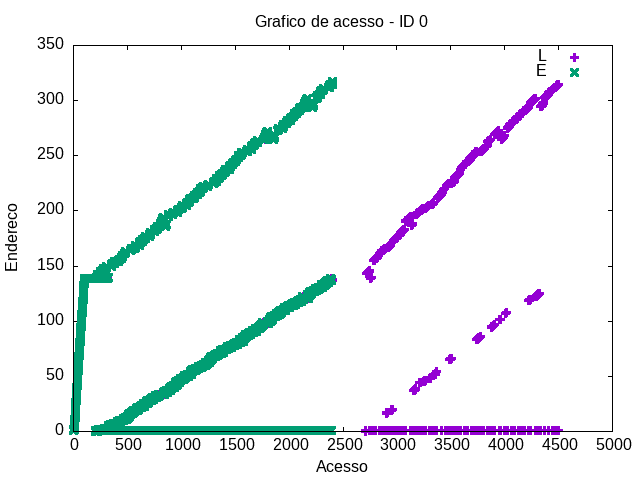
\includegraphics[width=\textwidth]{./images/100-200/common/registro_a-acesso-0.png}
        \caption{Acesso de memória do grafo}
        \label{fig:ac01}
    \end{subfigure}%
    \hfill
    \begin{subfigure}[c]{0.4\linewidth}
        \centering
        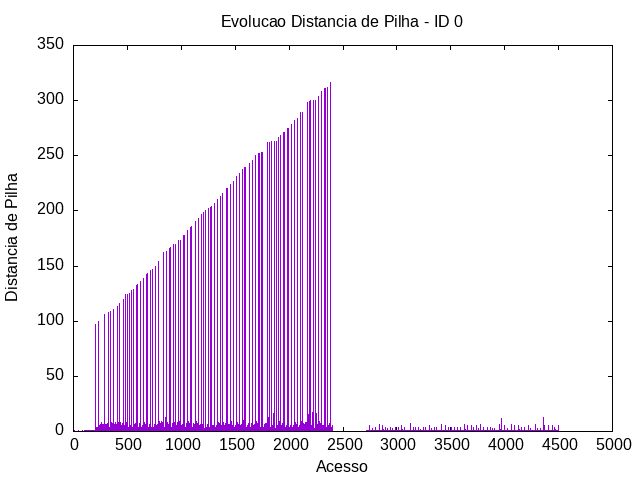
\includegraphics[width=\textwidth]{./images/100-200/common/registro_a-distp-0.png}
        \caption{Distância da pilha na leitura dos dados}
        \label{fig:ac02}
    \end{subfigure}
    \hfill
    \caption{Leitura dos dados}
\end{figure}

Nada de muito interessante aqui, tanto que me ambas as figuras podemos observar que na metade a esquerda do gráfico a leitura dos vértices e seus adjacentes e na segunda metade a leitura do grafo para verificar a gulosidade.
        
\subsubsection{Verificação de Gulosidade}

\begin{figure}[H]
    \centering
    \hfill
    \begin{subfigure}[c]{0.4\textwidth}
        \centering
        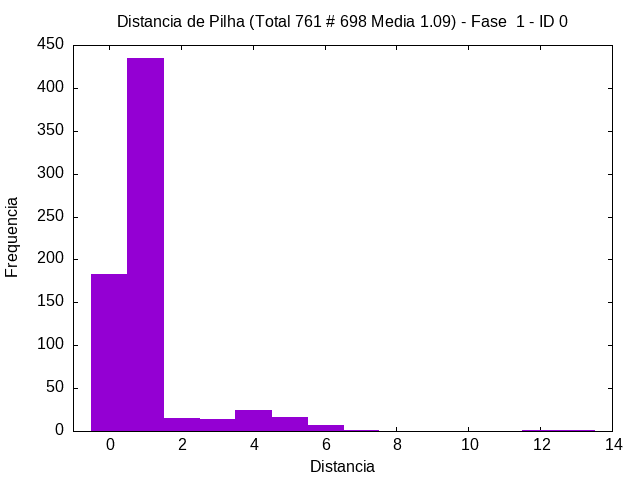
\includegraphics[width=\textwidth]{./images/100-200/common/registro_a-hist-1-0.png}
        \caption{Lista de adjacência do grafo}
        \label{fig:ac03}
    \end{subfigure}
    \hfill
    \begin{subfigure}[c]{0.4\textwidth}
        \centering
        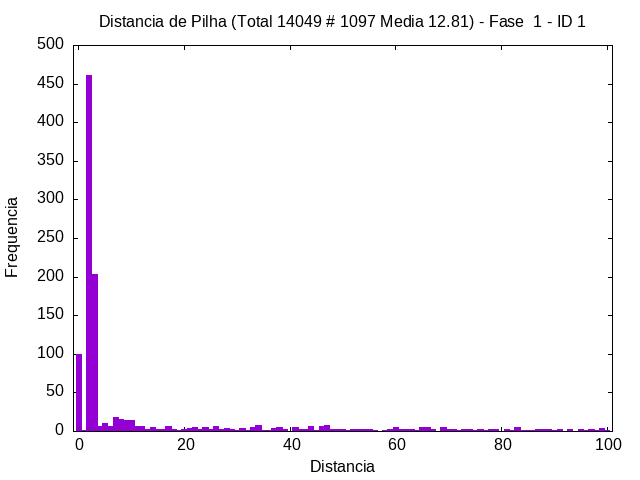
\includegraphics[width=\textwidth]{./images/100-200/common/registro_a-hist-1-1.png}
        \caption{Vetor de cores}
        \label{fig:ac04}
    \end{subfigure}
    \hfill
    \caption{Frequência de distância de pilha na verificação de gulosidade}

\end{figure}

\subsubsection{Ordenação}


\begin{figure}[H]
    \centering
    \hfill
    \begin{subfigure}[c]{0.4\textwidth}
        \centering
        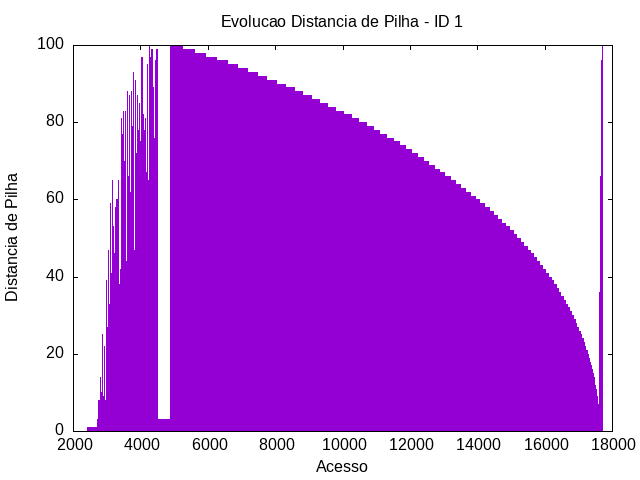
\includegraphics[width=\textwidth]{./images/100-200/bubblesort/registro_a-distp-1.png}
        \caption{Lista de adjacência do grafo}
        \label{fig:ac05}
    \end{subfigure}
    \hfill
    \begin{subfigure}[c]{0.4\textwidth}
        \centering
        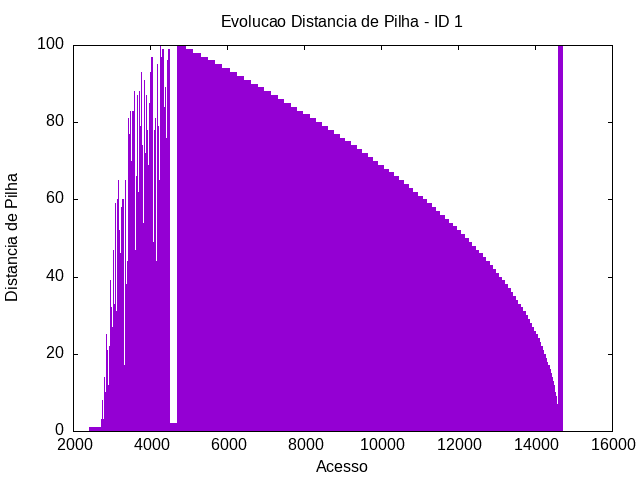
\includegraphics[width=\textwidth]{./images/100-200/selectionsort/registro_a-distp-1.png}
        \caption{Lista de adjacência do grafo}
        \label{fig:ac06}
    \end{subfigure}
    \hfill
    \begin{subfigure}[c]{0.4\textwidth}
        \centering
        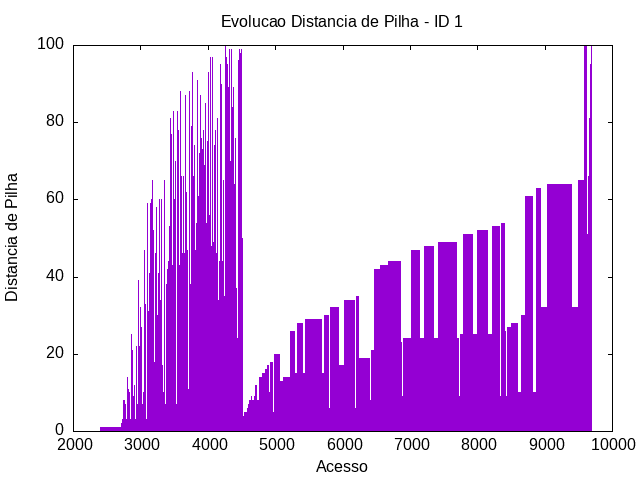
\includegraphics[width=\textwidth]{./images/100-200/inserctionsort/registro_a-distp-1.png}
        \caption{Lista de adjacência do grafo}
        \label{fig:ac07}
    \end{subfigure}
    \hfill
    \begin{subfigure}[c]{0.4\textwidth}
        \centering
        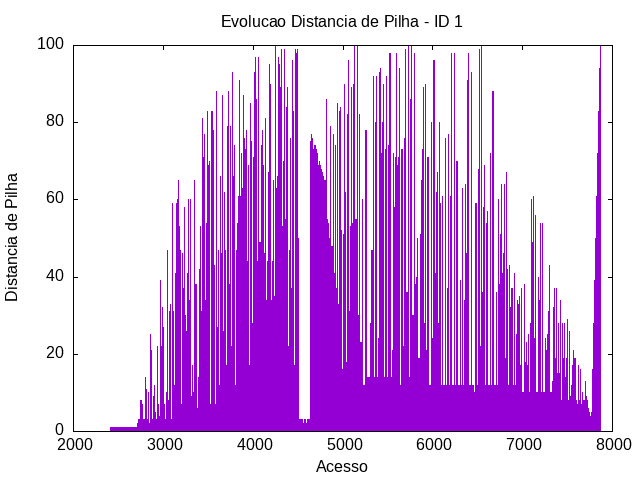
\includegraphics[width=\textwidth]{./images/100-200/heapsort/registro_a-distp-1.png}
        \caption{Lista de adjacência do grafo}
        \label{fig:ac08}
    \end{subfigure}
    \hfill
    \begin{subfigure}[c]{0.4\textwidth}
        \centering
        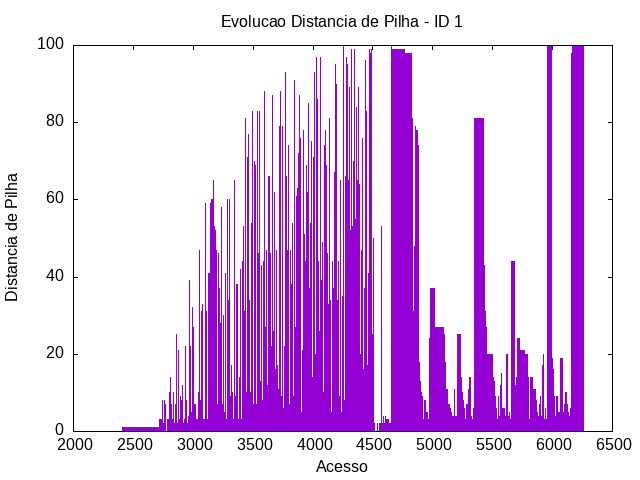
\includegraphics[width=\textwidth]{./images/100-200/quickSort/registro_a-distp-1.png}
        \caption{Lista de adjacência do grafo}
        \label{fig:ac09}
    \end{subfigure}
    \hfill
    \begin{subfigure}[c]{0.4\textwidth}
        \centering
        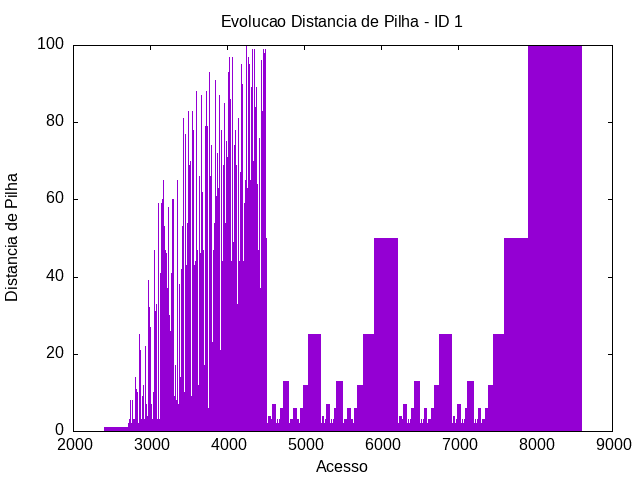
\includegraphics[width=\textwidth]{./images/100-200/mergesort/registro_a-distp-1.png}
        \caption{Lista de adjacência do grafo}
        \label{fig:ac10}
    \end{subfigure}
    \hfill
    \begin{subfigure}[c]{0.4\textwidth}
        \centering
        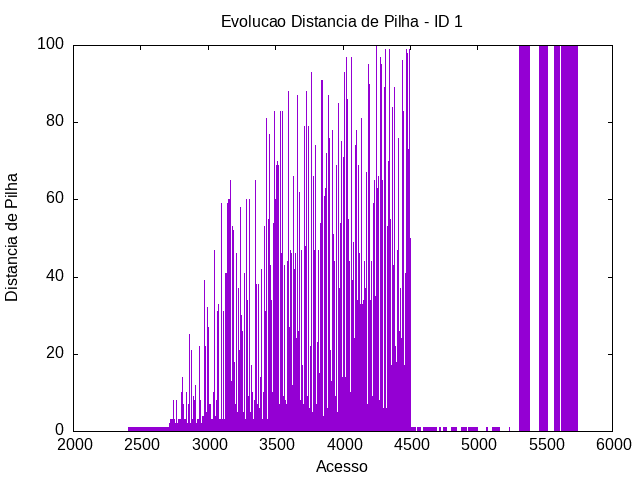
\includegraphics[width=\textwidth]{./images/100-200/my_sort/registro_a-distp-1.png}
        \caption{Lista de adjacência do grafo}
        \label{fig:ac05}
    \end{subfigure}
    \hfill
    \caption{Frequência de distância de pilha na verificação de gulosidade}

\end{figure}


% \begin{figure}[H]
    %     \centering
    %     \hfill
    %     \begin{subfigure}[c]{0.4\textwidth}
        %         \centering
        %         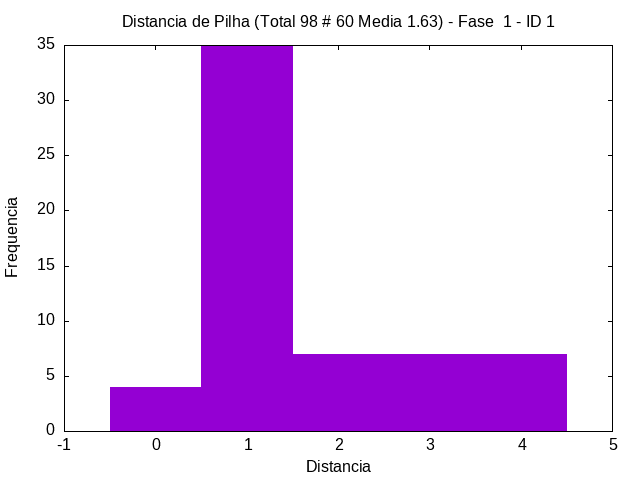
\includegraphics[width=\textwidth]{./images/sat_tree/registro_s-hist-1-1.png}
        %         \caption{Pilha da função evaluateExpression}
        %         \label{fig:ac05}
        %     \end{subfigure}
        %     \hfill
        %     \begin{subfigure}[c]{0.4\textwidth}
            %         \centering
            %         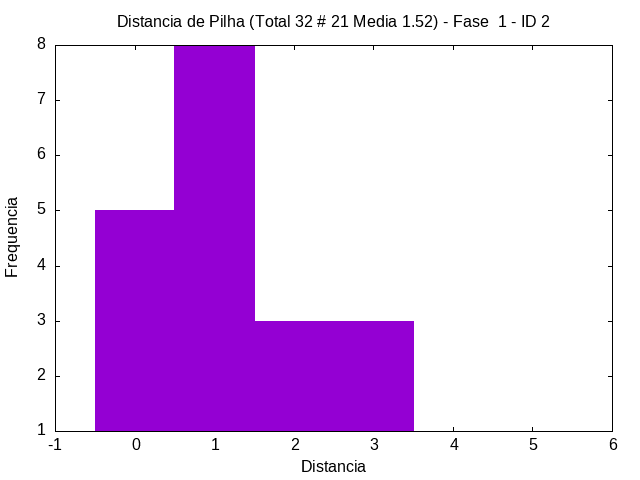
\includegraphics[width=\textwidth]{./images/sat_tree/registro_s-hist-1-2.png}
            %         \caption{Pilha da função sat\_tree}
            %         \label{fig:ac06}
            %     \end{subfigure}
            %     \hfill
            %     \caption{Distância da pilha}
            % \end{figure}
        % \end{figure}
            
            \subsection{Tempo de execução}
            
            Nesse experimento foi realizado medições de tempo de execução a parte de satisfatibilidade do programa, variando o número de quantificadores da expressão. Para isso,
            variamos a quantidade de quantificadores da expressão de 13 até 20, para que possamos observar o comportamento do programa para um número maior de quantificadores.
            Teve como base o seguinte comando (Atente-se que estamos variando o número de quantificadores): 


\verb#bin/tp01 -s "0 | 1 | 2 | (...) | 17 | 18 | 19" eeeeeeeeeeeeeeeeeeee#

% \begin{figure}[H]
    %     \centering
    %     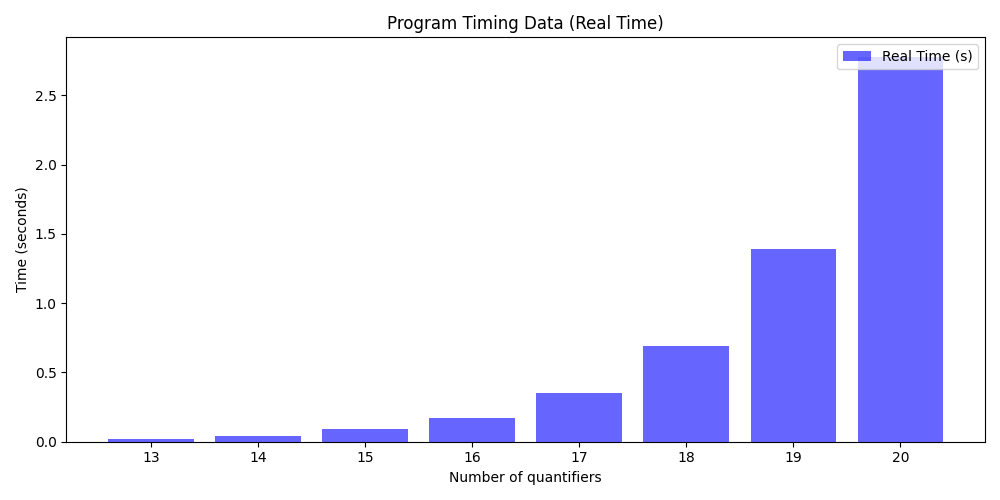
\includegraphics[width=0.6\textwidth]{./images/time.png}
    %     \caption{Tempo de execução do programa para diferentes números de quantificadores}
    %     \label{fig:time}
    % \end{figure}
    

Observa-se, portanto, comportamento semelhando a ordem de complexidade descrita anteriormente ($O(2^k)$), onde $k$ é o número de quantificadores.

\section{Conclusões}

O trabalho proposto foi de grande valia para o aprendizado de estruturas de dados, e de como elas podem ser utilizadas para solucionar problemas, afinal foi de extrema importância a utilização de pilhas e árvores como estruturas principais.  

Além disso, podemos observar que a análise de complexidade de grande importância, uma vez que ela nos permite prever o comportamento do programa para diferentes entradas, e assim, podemos realizar otimizações no código, como por exemplo, a utilização de uma estrutura de dados mais eficiente. Nesse trabalho, por exemplo, o problema de satisfatibilidade é um problema NP (determinístico não polinomial), ou seja, não existe uma solução conhecida em tempo polinomial, o que condiz com a solução implementada (de complexidade exponencial).

Por fim, a análise do tempo de execução de forma experimental foi de fato interessante pois permitiu conferir a similaridade com a teoria e o mundo real.
\section*{Bibliografia}

Slides da disciplina de Estrutura de Dados, ministrada pelo Prof. Wagner Meira Jr. e Prof. Eder Fereira Figuiredo.


\section*{Instruções para compilação e execução}

Em um terminal, navegue até a pasta raiz do projeto e execute os seguintes comandos:

\begin{verbatim}
    $ make
    $ ./bin/tp1.out -a "<expressão booleana>" <valores das variáveis> // Valor 
    $ ./bin/tp1.out -s "<expressão booleana>" <valores das variáveis> // SAT
\end{verbatim}

\end{document}